
%(BEGIN_QUESTION)
% Copyright 2008, Tony R. Kuphaldt, released under the Creative Commons Attribution License (v 1.0)
% This means you may do almost anything with this work of mine, so long as you give me proper credit

The following table shows recommended PID tuning settings for different process characteristic types.  The graph segments shown in the left-most column of the table characterize each process according to response to an open-loop (manual mode) step-change in controller output:

$$\includegraphics[width=15.5cm]{i03375x01.eps}$$

These recommendations must be altered, however, in the presence of substantial process noise.  Identify which control modes are affected by process noise (P, I, and/or D) and explain why.

\underbar{file i03375}
%(END_QUESTION)





%(BEGIN_ANSWER)

Process noise affects P and D control modes, but not I.
 
%(END_ANSWER)





%(BEGIN_NOTES)

Proportional control (P) directly repeats process noise to the output, multiplied by the gain setting.  Derivative control goes berserk with process noise, given the extremely high rates of change that noise represents.

%INDEX% Control, PID tuning: typical settings for different process types

%(END_NOTES)


